\documentclass[twocolumn]{article}

%Packages
\usepackage{amsmath}
\usepackage{amstext}
\usepackage{amssymb}
\usepackage{appendix}
\usepackage{coseoul}
\usepackage{enumerate}
\usepackage{graphicx}
\usepackage{import}
\usepackage{lscape}
\usepackage{modular}

\usepackage[pdfpagemode=UseNone,pdfstartview=FitH,colorlinks=true,linkcolor=blue,citecolor=blue,urlcolor=blue]{hyperref}
\usepackage[all]{hypcap}


% General physics constructs
\newcommand{\bra}[1]{\langle #1 |}
\newcommand{\ket}[1]{| #1 \rangle }
\newcommand{\braket}[2]{\langle #1|#2\rangle}
\newcommand{\bbraket}[3]{ \langle #1 | #2 | #3 \rangle }
\newcommand{\norm}[1]{\| #1\|}
\newcommand{\avg}[1]{\left \langle #1 \right \rangle}
\newcommand{\angavg}[1]{\left \langle #1 \right \rangle}
\newcommand{\abs}[1]{\left \lvert #1 \right \rvert}
\newcommand{\VS}{\textit{\textbf{V}}}
\newcommand{\Tr}{\textrm{Tr}}
\renewcommand{\Re}{\textrm{Re}}
\renewcommand{\Im}{\textrm{Im}}
\newcommand{\basis}[1]{\{\ket{#1}\}}

\newcommand{\omegaqubit}{\omega_{10}}

% Figures. Example usage:
% \quickfig{\columnwidth}{my_image}{This is the caption}{fig:my_fig}
\DeclareRobustCommand{\quickfig}[4]{
\begin{figure}
\begin{centering}
\includegraphics[width=#1]{#2}
\par\end{centering}
\caption{#3}
\label{#4}
\end{figure}
}

\DeclareRobustCommand{\quickwidefig}[4]{
\begin{figure*}[h]
\begin{centering}
\includegraphics[width=#1]{#2}
\par\end{centering}
\caption{#3}
\label{#4}
\end{figure*}
}


\title{Transmon}
\author{Daniel Sank \\
\small{University of California, Santa Barbara}\\
\small{presently Google Quantum AI}}
\date{28 April 2011}

\begin{document}

\maketitle

\section{Hamiltonian}
The Hamiltonian of the transmon with a single junction is
\begin{equation}
H = \frac{Q^2}{2C} - E_J \cos(2 \pi \Phi/\Phi_0)
\end{equation}
where $C$ is the total capacitance across the junction, $E_J = I_c \Phi_0 / 2\pi$ is the junction energy scale, $I_c$ is the junction critical current, $Q$ is the charge difference across the junction and $\Phi$ is the flux.
Note that $Q$ and $\Phi$ are cononically conjugate, ie. $[\Phi, Q] = i\hbar$.
This is frequently written in terms of the number of Cooper pairs $n$ that have tunnelled through the junction and the superconducting phase difference $\delta$,
\begin{equation}
H = 4 E_C n^2 - E_J \cos(\delta)
\end{equation}
where $n \equiv Q/2e$, $\delta = 2\pi \Phi/\Phi_0$, and $E_C = e^2/2C$. In this form the commutator is $[\delta, n] = i$.

\section{Numerical Analysis}
In order to solve the Hamiltonian numerically we must express it as a matrix in some basis.
Using $Q = -i \hbar (d/d\Phi)$ and $\Phi_0 \equiv h/2e$, we can express the Hamiltonian as a differential operator in the $\delta$ basis,
\begin{equation}
H = -4 E_C \frac{d^2}{d\delta^2} - E_J \cos(\delta) \, .
\end{equation}
We now discretize the position variable $\delta$ into $N$ points such that the distance between position points is $d\delta = 2\pi/N-1$. In this discretized basis the second derivative is a matrix,
\begin{equation}
S_{ij} = \frac{1}{d\delta^2} \left( -2\delta_{ij} + \delta_{i,j+1} + \delta_{i,j-1} \right) \end{equation}
and the Hamiltonian is \begin{equation}
H_{ij}/E_C = -4\,S_{ij} - \left( \frac{E_J}{E_C} \right) \cos(j \, d\delta) \delta_{ij} \end{equation}
This matrix can be diagonalized numerically. This is done in a program located at "pyle/sim/transmon.py". The first few energy eigenstates are plotted in the $\delta$ basis in Fig. \ref{Fig:wavefunctions}

The utility of this numerical solution is that it can be inverted so that a measurement of the qubit frequency and anharmonicity at the insensitive point immediately yield exact values for $E_{J_0}$ and $E_C$. The code to do this inversion is in the file mentioned above.

\begin{figure}
\begin{centering}
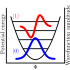
\includegraphics[width=9cm]{wavefunctions.pdf} 
\par\end{centering}
\caption{The first three transmon wavefunctions}
\label{Fig:wavefunctions}
\end{figure}

%\begin{figure}
%\begin{centering}
%\includegraphics[width=9cm]{relativeAnharmonicity.eps} 
%\par\end{centering}
%\caption{Relative anharmonicity of the transmon as a function of $E_J/E_C$}
%\label{Fig:relativeAnharmonicity}
%\end{figure}

\section{Perterbative Analysis}

Approximate results for the transmon can be obtained through perturbation theory.
Since the transmon operates in the regime $E_J/E_C \gg 1$ the width of the wavefunctions is small and the cosine potential can be approximated as a quartic
\begin{equation}
H = 4E_C n^2 - E_J \left(1 - \frac{\delta^2}{2} + \frac{\delta^4}{24} + \cdots \right) \, .
\end{equation}
This can be separated into a harmonic part and a perturbing quartic
\begin{align}
H =& H_0 + V \\
\textrm{where} \quad H_0  =& 4E_C n^2 + \frac{E_J}{2} \delta^2 \\
V =& -\frac{E_J}{24} \delta^ 4 \, .
\end{align}
The solution to the harmonic part is well know.
Using the notation from my harmonic oscillator cheat sheet we have \begin{equation}
u = \delta \quad v = n \quad \alpha = E_J \quad \beta = 8E_C \quad \gamma = 1 \end{equation}
from which we get the harmonic or ``plasma'' resonance frequency
\begin{equation}
f_p \equiv \gamma \sqrt{\alpha \beta}/h = \sqrt{8 E_C E_J}/h = \frac{1}{2\pi} \sqrt{\frac{1}{L_J C}} \label{eq:plasmaFreqInEnergy}
\end{equation}
where $L_J \equiv \Phi_0 / (2\pi I_c)$ is the junction characteristic inductance.
Defining frequencies $f_C \equiv E_C/h$ and $f_J \equiv E_J/h$, Eq. (\ref{eq:plasmaFreqInEnergy}) can be rewritten as
\begin{equation}
f_p = \sqrt{8 f_C f_J} \label{eq:plasmaFrequency}
\end{equation}
which is more useful than the version with $E_J$ and $E_C$ because in real life physicists almost never think about physical quantities with dimensions of energy, i.e. you can't measure energy in the lab.

The perturbation calculation is easiest with raising and lowering operators.
Using the cheat sheet again we get \begin{eqnarray}
u &=& \sqrt{\gamma} \left( \frac{\beta}{\alpha} \right) ^{1/4} \frac{1}{\sqrt{2}} (a + a^{\dagger}) \\
\delta &=& \left( \frac{8E_C}{E_J} \right) ^{1/4} \frac{1}{\sqrt{2}} (a + a^{\dagger}) \\
\textrm{so} \quad V &=& -\frac{E_C}{12} (a + a^{\dagger})^4 \end{eqnarray}
Grinding through first order perturbation theory gives you the following (first order) level shifts \begin{equation}
\delta E_0^{(1)} = -E_C \frac{1}{4} \quad \delta E_1^{(1)} = -E_C \frac{5}{4} \quad \delta E_2^{(1)} = -E_C \frac{13}{4}\end{equation}
resulting in \begin{eqnarray}
f_{10} &=& f_p - f_C \\
f_{21} &=& f_{10} - f_C \end{eqnarray}
which agrees with the Koch paper.
Note that the anharmonicity is
\begin{equation}
\eta/2\pi \equiv f_{21} - f_{10} = -f_C \, .
\end{equation}
In other words, the frequency scale of capacitor is the anharmonicity.

\section{Flux Tuning}
The transmon junction is actually a dc SQUID which has inductance tuned by external flux.
The inductance of the SQUID loop depends on the flux $\Phi_\text{sq}$ threading the SQUID as
\begin{equation}
L_J(\Phi_\text{sq}) = L_{J_0} \sec \left( \pi \Phi_\text{sq} / \Phi_0 \right) \, .
\end{equation}
Using $E_J = (\Phi_0/2\pi)^2 / L_J$ we infer the Hamiltonian
\begin{equation}
H = \frac{Q^2}{2C} - E_{J_0} \cos(\pi \Phi_\text{sq} / \Phi_0) \cos(2\pi \Phi / \Phi_0) \, .
\end{equation}
Therefore, the transmon frequency depends on external flux according to
\begin{align}
f_{10}
= & \frac{1}{2 \pi \sqrt{L_{J_0} C}} \cos \left( \pi \varphi \right)^{1/2} - f_C \\
= & \sqrt{8 f_{J_0} f_C} \cos \left( \pi \varphi \right)^{1/2} - f_C \\
= & f_{p_0} \cos \left( \pi \varphi \right)^{1/2} - f_C \, .
 \label{eq:freqVsFluxI}
\end{align}
The two parameters $f_{J_0}$ and $f_C$ can be determined exactly once the qubit's frequency and anharmonicity are known at the flux insensitive point, so there are no free parameters in Eq. (\ref{eq:freqVsFluxI}).

\subsection{How to Measure Flux sensitivity}
In the lab we do not directly control bias flux. Instead, we control the value of a digitally controlled voltage source.
Writing the bias flux in terms of the actual voltage control parameter, and adding an arbitrary environmentally induced flux offset, we get \begin{equation}
f_{10} = \sqrt{8 f_J f_C} \cos \left( \pi \frac{M}{\Phi_0 Z} V - \pi \frac{\Phi_{\textrm{offs}}}{\Phi_0} \right)^{1/2} - f_C \end{equation}
Here $Z$ if the effective resistance of the bias line. If this is a microwave line this impedance has to be computed carefully, taking attenuators into account correctly. If we measure the transmon frequency against $V$ we can fit for the two combinations of parameters $\pi M / \Phi_0 Z$ and $\Phi_{\textrm{offs}} / \Phi_0$.


\section{Dephasing}

In this section we discuss limits on the qubit's phase coherence time from bias noise and other effects. The decay curve for a Ramsey experiment is given by \begin{equation}
p(t) = \exp -2\pi^2 \left( \frac{df_{10}}{d\lambda} \right)^2 t \int_{f_{min}t}^{f_{max}t}S_{\lambda}\left(\frac{z}{t}\right)\left( \frac{\sin(\pi z)}{\pi z} \right)^2 dz \label{eq:ramseyDecay} \end{equation}
In general the qubit frequency depends on capacitance, junction intrinsic critical current, and flux bias. The control electronics only couple to flux so we take $\lambda \rightarrow \Phi$ from here on.

We can write the noise spectral density as \begin{equation}
S_{\Phi}(f) = \frac{S^*_{\Phi}1\textrm{Hz}^{\alpha}}{f^{\alpha}} \end{equation}
where $S^*_{\Phi}$ is the flux noise spectral density at 1Hz. Inserting this into eq. (\ref{eq:ramseyDecay}) the integral becomes \begin{equation}
S^*_{\Phi} \times (10^{-9} t \textrm{GHz})^{\alpha} \int_{f_{min}t}^{f_{max}t}\left( \frac{\sin(\pi z)}{\pi z}\right)^2 \frac{dz}{z^{\alpha}} \end{equation}
Denoting \begin{equation}
I(\alpha, t) = (10^{-9}t\,\textrm{GHz})^{\alpha} \int_{f_{min}t}^{f_{max}t} \left(\frac{\sin(\pi z)}{\pi z}\right)^2 \frac{dz}{z^{\alpha}}
\end{equation}
we get \begin{equation}
p(t) = \exp -2\pi^2 \left( \frac{df_{10}}{d\lambda} \right)^2 t S_{\Phi}^* I(\alpha, t) \end{equation}
Let $x = f_{10}(\Phi)/f_{10}(0)$ and define a quantity $\Delta(x)$ by the equation \begin{equation}
\left( \frac{df_{10}(\Phi)}{d\Phi} \right) = \frac{f_{10}(0)}{\Phi_0}\Delta(x) \end{equation}
With this definition we have \begin{equation}
p(t) = \exp -2\pi^2 \Delta(x)^2 f_{10}(0)^2 t \frac{S_{\Phi}^*}{\Phi_0^2} I(\alpha,t) \end{equation}
Since the qubit is a short at frequencies relevant to bias noise the flux noise induced by the bias electronics can be written as \begin{equation}
S^*_{\Phi} = \left(\frac{V^*_{model}M}{R}\right)^2 \end{equation}
Here $V^*_{model}$ is the voltage noise per square root frequency at 1Hz and $R$ is the output resistance of a model circuit for the bias electronics. These numbers are derived quite differently for a low impedance output circuit like the fastbias and a 50 Ohm circuit like the GHz DACs, and details are given below. Define $v^*$, $m$, and $r$ by the following equations: \begin{eqnarray}
V^*_{model} &=& v^*\times \frac{nV}{\sqrt{\textrm{Hz}}} \nonumber \\
M &=& m\times\textrm{pH} \nonumber \\
R &=& r \times \textrm{Ohm} \nonumber \end{eqnarray}
With these definitions we have \begin{equation}
\frac{S^*_{\Phi}}{\Phi_0^2} = \left( \frac{v^*m}{2r} \right)^2 \frac{10^{-3}}{\textrm{GHz}} \end{equation}
and therefore \begin{equation}
p(t) = \exp -2\pi^2 \Delta(x)^2 f^2 t_{ns} \left(\frac{v^* m}{2r} \right)^2 10^{-3} I(\alpha,t) \end{equation}
where here $f = f_{10}(0)/\textrm{GHz}$.

\subsection{Qubit Sensitivity}

We develop a simple formula relating the qubit's sensitivity $df_{10}/d\Phi$ to operating condition. The qubit frequency as a function of bias flux is given by Eq. (\ref{eq:freqVsFluxI}). Note that the unbiased frequency is $f_{10}(0) = f_{p0} - f_C$, so \begin{eqnarray*}
f_{10}(\Phi) &=& (f_{10}(0)+f_C)\cos \left( \pi \Phi/\Phi_0 \right)^{1/2} - f_C \\
&=& f_{10}(0)\cos \left( \pi \Phi/\Phi_0 \right)^{1/2} + \left( \cos \left( \pi \Phi/\Phi_0 \right)^{1/2} - 1\right)f_C \\
&\approx& f_{10}\cos \left( \pi \Phi/\Phi_0 \right)^{1/2} \end{eqnarray*}
Differentiating, we get \begin{equation}
\frac{df_{10}(\Phi)}{d\Phi} \approx - \frac{\pi}{2}\frac{f_{10}(0)}{\Phi_0}\left(\frac{f_{10}(0)}{f_{10}(\Phi)}\right) \left[1- \left(\frac{f_{10}(\Phi)}{f_{10}(0)}\right)^4 \right]^{1/2} \end{equation}
or in dimensionless units \begin{equation}
\frac{df_{10}(\Phi)/d\Phi}{f_{10}(0)/\Phi_0} = -\frac{\pi}{2}\frac{f_{10}(0)}{f_{10}(\Phi)} \left[1- \left(\frac{f_{10}(\Phi)}{f_{10}(0)}\right)^4 \right]^{1/2} \label{eq:transmonSensitivity} \end{equation}
This function is plotted in Fig. \ref{Fig:transmonSensitivity}. In the notation defined above this result is equivalent to \begin{equation}
\Delta(x) = -\frac{\pi}{2}\frac{1}{x}\left( 1 - x^4 \right)^{1/2} \end{equation}

\begin{figure}
\begin{centering}
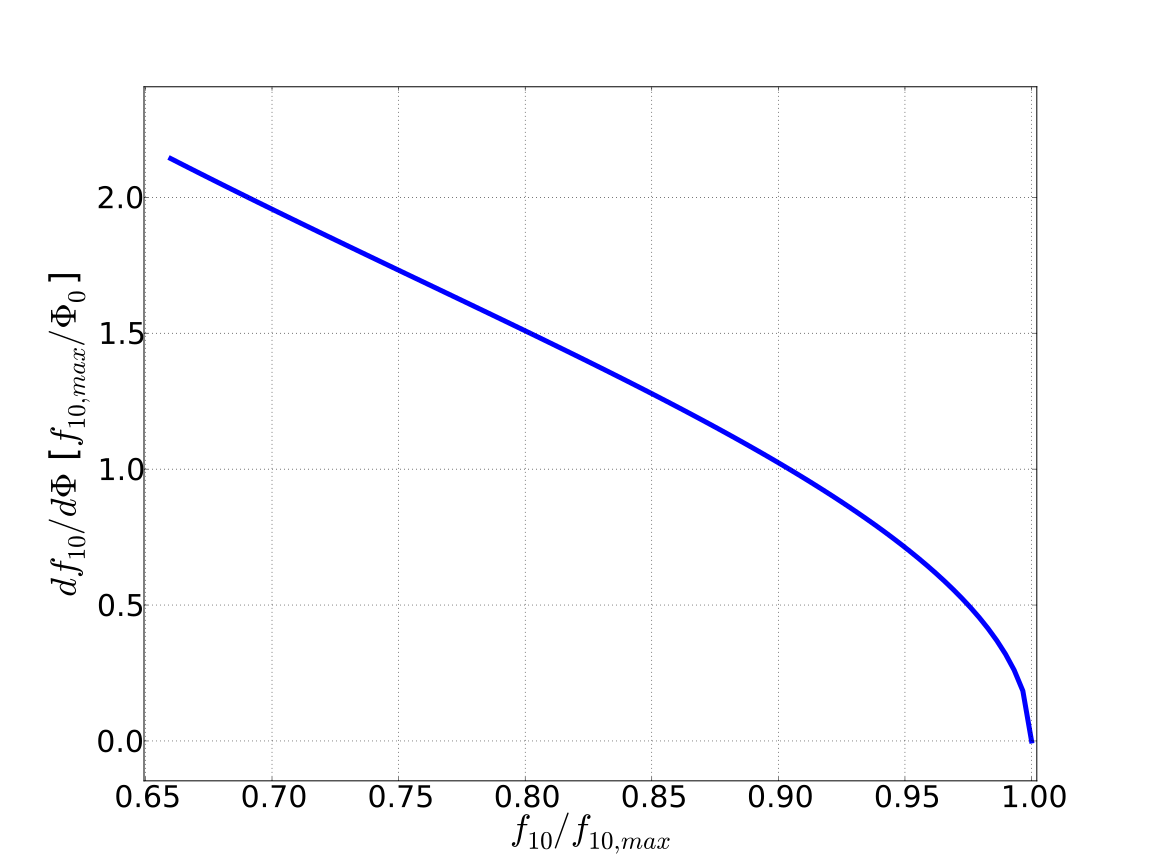
\includegraphics[width=9cm]{transmonSensitivity.pdf} 
\par\end{centering}
\caption{Sensitivity of transmon to bias flux}
\label{Fig:transmonSensitivity}
\end{figure}

\subsection{Bias noise from 50 $\Omega$ source}

The voltage noise of a 50$\Omega$ source is characterized by the voltage fluctuations measured at a matched load. The model for the noise source must therefore have a source voltage of twice the measured voltage, with an output resistance of 50$\Omega$. For example, if we measure 6nV/rtHz noise, the source is modelled with 12nV/rtHz internal noise voltage, in series with a 50$\Omega$ resistor. If attenuators are placed in line with the source, the noise is reduced. If the attenuation is 0dB, then the power delivered to the load is $\frac{1}{2}V^2/R$. Addition of the attenuators reduces this to $\frac{1}{2}V^2 10^{-N/10}/R$. Since the source plus attenuators are still a matched source, we can model it as a new source with voltage $V'$ and output impedance of 50$\Omega$. The new voltage is found by noting that the power delivered to the load must be $\frac{1}{2}V'^2/R$, giving \begin{equation}
V' = V 10^{-N/20} \end{equation}
Note that the source voltage is twice $V'$. The formula for the model source voltage is therefore \begin{equation}
V_{model} = 2V' = 2 V_{measured} 10^{-N/20} \label{eq:50OhmSourceVoltage} \end{equation}


\subsection{White noise}

For white noise with an upper cutoff at $f_{max}$ the power $\alpha=0$ and we get \begin{equation}
I(\alpha, t) = \frac{1}{2+(f_{max}t)^{-1}} \end{equation}


\subsection{$1/f$ noise}

For $1/f$ noise the lower cutoff $f_{min}$ we have $\alpha=1$ and \begin{equation}
I(\alpha, t) = 10^{-9} t_{ns} \ln \left( \frac{0.4}{f_{min}t}\right) \end{equation}

\subsection{Qubit Tuning}
Our GHz DAC plus differential amplifier has an output range of -360mV to +360mV. With $N$ dB attenuation on the line, this gives a current bias range of \begin{equation}
\pm V_{\textrm{model}}/R = \pm 2 \frac{V_{\textrm{meas}}}{R} 10^{-N/20} = \pm 15.2\textrm{mA}\,\,10^{-N/20} \end{equation}
The available frustration range is therefore \begin{equation}
f = \frac{\Phi}{\Phi_0} = \frac{IM}{\Phi_0} \approx \pm 7.6 m\,\, 10^{-N/20} \end{equation}
where here $m$ is the mutual inductance of the bias line in pH. Using another bias source (fastbias) to idle away from the flux insensitive point we could dynamically access a range of frustrations from 0 to $2f$, giving a lowest accessible frequency of $f_{10}(0) \cos \left( \pi 2f \right)^{1/2}$.  For $N=40$ the minimum accessible frequency is 76\% of the maximum. With a flux insensitive point frequency of 7GHz you could go down to 5.3GHz. With instead 30dB attenuation it would be possible to access the entire frequency range of the transmon.


\end{document}
